\subsection{Sequence Diagram}

\begin{figure}[H]
    \centering
    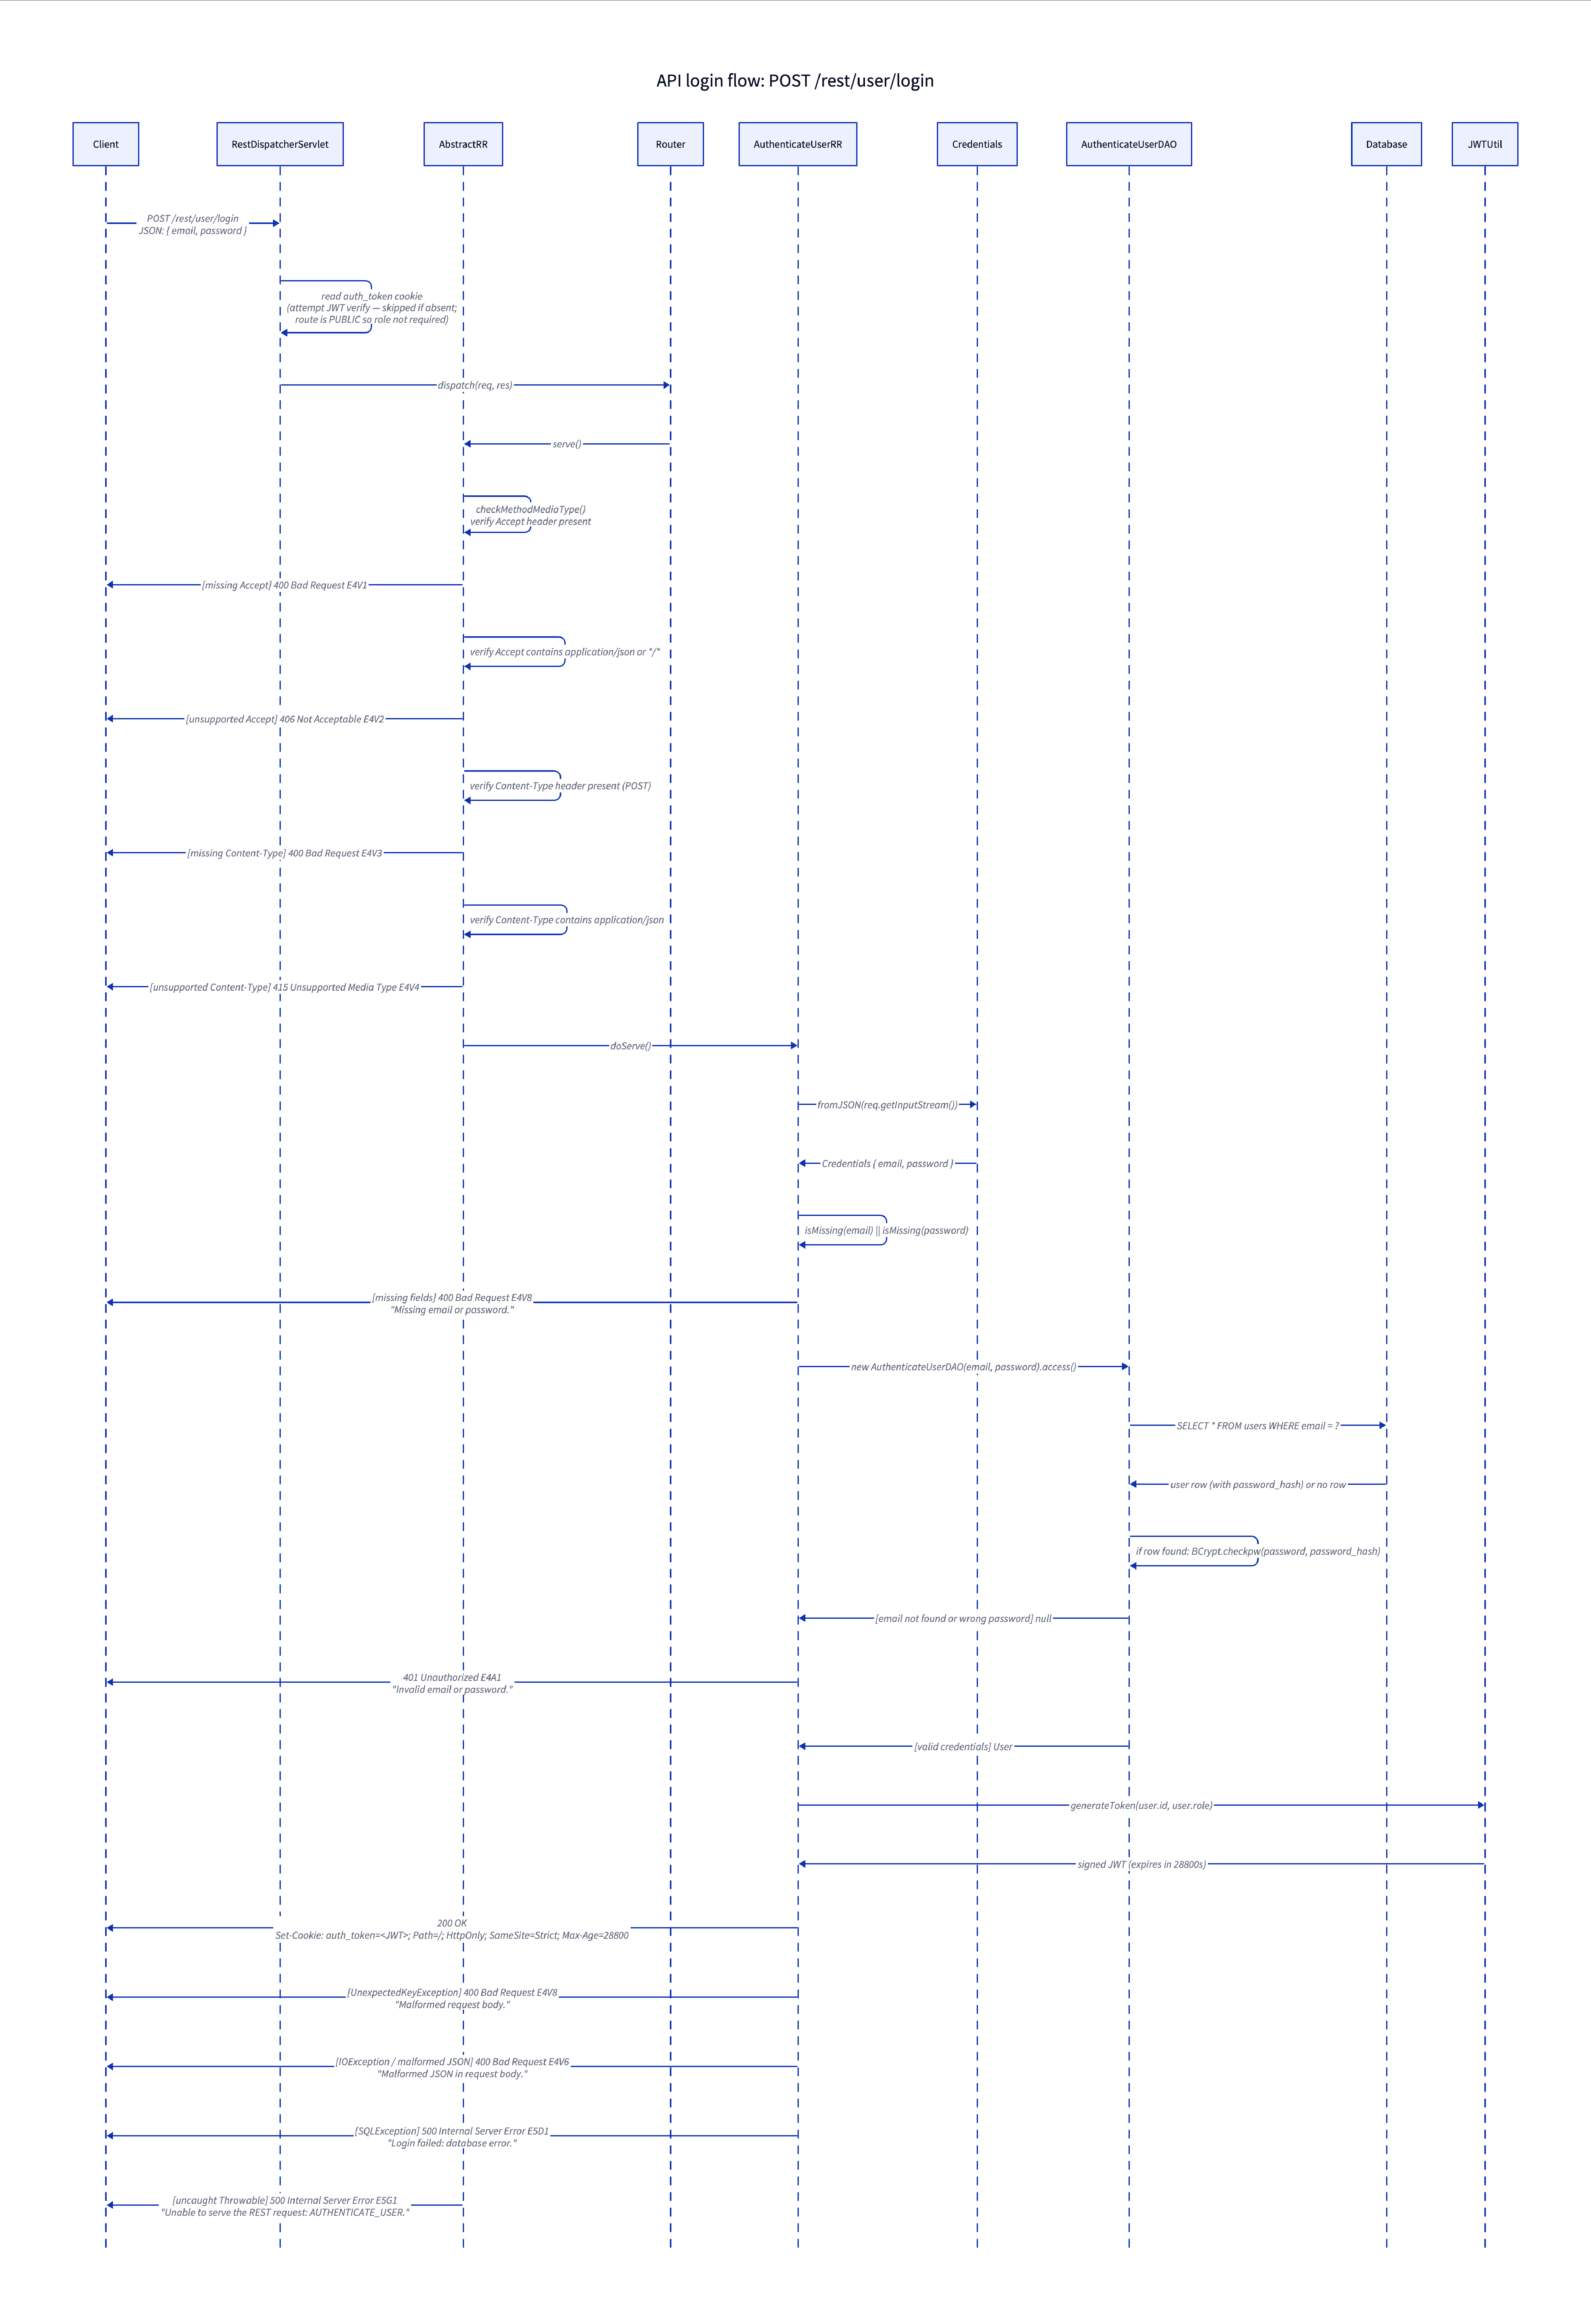
\includegraphics[width=0.9\textwidth]{images/sequence_diagram.pdf}
    \caption{Home page's mockup}
    \label{fig:Home page's mockup}
\end{figure}

The following three examples are representative of how the application processes HTTP requests. The first shows user registration, the second shows user login, and the third shows how an authenticated request to the dashboard is handled by the \texttt{AuthFilter}.

\subsubsection*{User Registration - POST /rest/user/register}

When a client sends a \texttt{POST} request to \texttt{/rest/user/register}, the Tomcat container receives it and forwards it to \texttt{RestDispatcherServlet}, which is the single entry point for all \texttt{/rest/*} requests. The dispatcher sets the client IP in \texttt{LogContext}, then uses its internal \texttt{Router} to match the method and path against registered routes and instantiates \texttt{RegisterUserRR}.

\texttt{RegisterUserRR.doServe()} first invokes \texttt{AbstractRR.checkMethodMediaType()} to verify that the \texttt{Accept} header contains \texttt{application/json} and that the \texttt{Content-Type} header is also \texttt{application/json}; if either check fails, an appropriate error \texttt{Message} is returned immediately with the corresponding error code (\texttt{E4V1}--\texttt{E4V5}). It then deserialises the request body into a \texttt{User} object via \texttt{User.fromJSON()}, which throws \texttt{MalformedJSONException} if an unexpected field is encountered. If any required field (username, email, password, name, surname, phone number) is missing or blank, a \texttt{400 Bad Request} response is returned with error code \texttt{E4V8}. If the email does not match the expected pattern or the password does not satisfy the security policy, the same error code is returned with a descriptive message.

If validation passes, a \texttt{RegisterUserDAO} is instantiated with the validated \texttt{User} object and \texttt{access()} is called. \texttt{AbstractDAO.access()} acquires a connection from \texttt{ConnectionPoolSingleton} and delegates to \texttt{RegisterUserDAO.doAccess()}, which hashes the plain-text password with \texttt{BCrypt.hashpw()} and executes an \texttt{INSERT} returning the generated user id. If the email, username, or phone number already exists, PostgreSQL raises a \texttt{23505} unique constraint violation; \texttt{RegisterUserRR} catches this and returns \texttt{409 Conflict} with error code \texttt{E4R3}. Any other \texttt{SQLException} yields \texttt{500 Internal Server Error} with error code \texttt{E5D1}. On success, \texttt{RegisterUserRR} sets the status to \texttt{201 Created} and serialises a \texttt{User} object containing only the new user's id.

\subsubsection*{User Authentication - POST /rest/user/login}

When a client sends a \texttt{POST} request to \texttt{/rest/user/login}, the dispatcher instantiates \texttt{AuthenticateUserRR}. After the standard MIME-type checks by \texttt{checkMethodMediaType()}, the handler deserialises the request body into a \texttt{Credentials} object via \texttt{Credentials.fromJSON()}, verifying that both \texttt{email} and \texttt{password} fields are present and non-blank. A \texttt{MalformedJSONException} is thrown if unexpected fields are found.

An \texttt{AuthenticateUserDAO} is instantiated with the provided email and password and \texttt{access()} is called. \texttt{doAccess()} executes \texttt{SELECT id, password\_hash FROM users WHERE email = ?}. If no row is found, \texttt{outputParam} remains \texttt{null}. If a row is found, \texttt{BCrypt.checkpw()} verifies the submitted password against the stored hash; on match, \texttt{outputParam} is set to the user's id. A \texttt{null} output param causes \texttt{AuthenticateUserRR} to return \texttt{401 Unauthorized} with error code \texttt{E4A1}. On success, \texttt{JWTUtil.generateToken(userId)} produces a signed HMAC-256 JWT containing the \texttt{user\_id} claim and an 8-hour expiry. The token is attached to the response via \texttt{Set-Cookie} with the flags \texttt{HttpOnly} and \texttt{SameSite=Strict}, and the status is set to \texttt{200 OK}.

\subsubsection*{Authenticated Dashboard Request - GET /dashboard/*}

When an authenticated user sends any request to a URL matching \texttt{/dashboard/*}, the Tomcat container intercepts it with the \texttt{AuthFilter} before reaching any servlet. The filter calls \texttt{extractTokenFromCookies()} to find the cookie named \texttt{auth\_token} among the request cookies. If no such cookie exists, the filter immediately calls \texttt{res.sendRedirect("/login")} and the chain is not invoked.

If the cookie is found, \texttt{JWTUtil.verify(token)} is called. This method uses the pre-initialised HMAC-256 verifier to check both the signature and the expiry time of the token. If verification throws a \texttt{JWTVerificationException} (invalid signature or expired token), the filter redirects to \texttt{/login} with error code \texttt{E4A3}. If verification succeeds, the \texttt{user\_id} claim is extracted from the decoded JWT and stored as a request attribute (\texttt{req.setAttribute("user\_id", userId)}). The filter then calls \texttt{chain.doFilter(request, response)}, passing the enriched request to the next component in the pipeline, which can read the \texttt{user\_id} attribute to identify the authenticated user without re-querying the database.